%%%%%%%%%%%%%%%%%%%%%%%%%%%%%
% Supplementary Information %
%%%%%%%%%%%%%%%%%%%%%%%%%%%%%
\captionsetup*{format=largeformat}
\section{JF549 dye photobleaching kinetics}
\label{note:dye_bleaching} 

In our approach to estimating RecB binding times to DSBs, the photostability of the fluorescent dye was of primary concern. Since we detect single molecules of RecB bound to DSBs, two main photophysical behaviours were liable to cause artefacts in our data:
\begin{enumerate}
    \item Photobleaching (an irreversible loss of fluorescence) would limit the maximum number of frames we can track a DSB-bound RecB for, and would artefactually reduce the fitted binding times since some fluorescent spots might disappear due to photobleaching rather than unbinding from DNA
    \item Blinking (a transient loss of fluorescence) could cause repeated disappearance and reappearance of single molecules, and hence bias the computed binding times
\end{enumerate}

To address these concerns, we computed ensemble-level photobleaching curves by integrating the total fluorescence signal from the cells (Supp. Fig. \ref{SIFig:dye_bleaching}A). After 50 frames of laser exposure, a significant amount of photobleaching was noticeable (27\% $\pm$ 9 of the initial fluorescence remaining). The exact photobleaching rate of the dye in our experimental conditions can be estimated by fitting the photobleaching curve with an exponential decay function of the form $y=a.e^{-k.t}+b$ (with a the amplitude of the fit, k the bleaching rate, and b an offset to account for cellular auto-fluorescence). Since the bleaching rate is expected to mostly depend on experimental parameters that vary between but not within datasets (output laser power, HiLo angle), one bleaching rate was computed per dataset (Supp. Fig. \ref{SIFig:dye_bleaching}B). The true RecB dissociation rates were computed by subtracting the corresponding bleaching rates from the fitted spot disappearance rates.

All experimental photobleaching curves were well-fitted by a mono-exponential decay function. If significant blinking of the dye was occurring, we would expect photobleaching curves to follow more complex kinetics \cite{Thedie2017}. We therefore concluded that in our experimental conditions, the JF549 dye was not experiencing blinking, consistent with previous reports of the dye's outstanding photostability \cite{Grimm2015}.

\section{Formation of RecB spots by the freely diffusing RecBCD-Halo-Gam complex}
\label{note:spurious_spots}
In cells that overexpress the Gam protein, RecB is expected to be unable to bind DSBs. Even though Gam overexpression prevents the apparition of long-lived RecB spots under exposure to ciprofloxacin, short-lived RecB spots remain present (Figure \ref{Fig:lifetimes}C, Supp. Figure \ref{SIFig:Gam_RecB_lifetimes_vs_WT} and Table \ref{tab:fit_results}). To understand how RecB spots can be formed in the absence of DSB binding, we simulated the expected displacements of a RecBCD-Halo-Gam complex according to the distribution of single displacements for a random 2D walk:
\begin{equation}
    P(r) = \dfrac{r}{2D_i t}e^{-\dfrac{r^2}{4D_i t}}
\end{equation}

with $D_i$ the apparent diffusion coefficient, and $t$ the frame time. Our previous work found a diffusion coefficient for RecB-Halo of $\sim$1.5 \ums\ \cite{Lepore2023}. Assuming that the diffusion coefficient of the complex (that does not interact with DSBs) is proportional to the cube of the molecular weight, we expect a diffusion coefficient for the full RecBCD-Halo-Gam complex (386 kDa, 353 kDa without the Gam protein) of $\sim$1 \ums. The frame time in our experiments is 1 second, but it is likely that a molecule that would stay immobile for a fraction of that time would still be visible as a spot. Although calculating a precise value is challenging, we used a ballpark estimate of 500 ms (half our frame time) of a molecule being immobile to be detected as a spot in our experiment. Supp. Figure \ref{SIFig:displacement_simul} shows the distribution of expected displacements under these parameters. Although most displacements would be too large to result in a bright fluorescent spot, a small fraction ($\sim$4\%) are smaller than 300 nm, and could create a spot. When factoring in the number of RecB molecules per cell (5 on average \cite{Lepore2019a}) and the number of frames in our timelapse (50), this would result in $\sim$10 RecB spots per cell, on the same order of magnitude as the number of spots observed in our experiments in the presence of the Gam protein (4.1 $\pm$ 0.2, mean $\pm$ sem). Note that a single RecB molecule can form several spots over the length of the timelapse experiment.

\clearpage

\setlength\intextsep{40pt}

%% SUPPLEMENTARY FIGURES

% Strains table
\begin{supptable}[htbp]
    \centering
    \caption{List of bacterial strains used in this study}
    \begin{tabular}{lll}
        \toprule
        Name & Description & Reference\\
        \midrule
        MEK2623 & MG1655 \textit{recB::halotag recA::syfp2} & this work\\
        MEK2622 & MG1655 \textit{recB::halotag $\Delta$recA} & this work \\ % = AL133_1
        MEK716 & MG1655 \textit{recB1080::halotag} & this work \\ % = AL139_3
        MEK2324 & MG1655 \textit{recB1080::halotag HK022::psfiA-GFP} & \cite{Lepore2023} \\
        MEK65 & MG1655 \textit{recB::halotag} & \cite{Lepore2019a} \\
        MEK2629 & MG1655 \textit{recB::halotag pBad::GamL} & this work \\ % = AL119
        DL654 & MG1655 \textit{$\Delta$recA} & \cite{Wertman1986} \\
        \bottomrule
    \end{tabular}
    \label{SItab:strains}
\end{supptable}

% Plasmids table
\begin{supptable}[htbp]
    \centering
    \caption{List of bacterial plasmids used in this study}
    \begin{tabular}{lll}
        \toprule
        Name & Description & Reference\\
        \midrule
        pSF1 & Expression of HaloTag under the control of the pBAD promoter & \cite{Lepore2019a} \\
        pDT6 & GamL inserted into pBAD322K by restriction cloning & \cite{Wilkinson2016} \\
        \bottomrule
    \end{tabular}
    \label{SItab:plasmids}
\end{supptable}

% Acquisition parameters table
\begin{supptable}[htbp]
    \centering
    \caption{Acquisition parameters used for microscopy.}
    \begin{tabular}{lllllll}
        \toprule
        Channel & Illumination & Intensity & Exposure (ms) & EM gain & Images (interval) & Z-stack\\
        \midrule
        Brightfield & Lamp & NA & 30 & 0 & 1 & 16 slices, 0.2 µm step\\
        JF549 & 561-nm & 2 mW & 1000 & 150 & 50 (2 sec) & No\\
        SYFP2 & 488-nm & 2 mW & 50 & 100 & 50 (2sec) & No\\
        Sytox Green & 488-nm & 2 mW & 50 & 100 & 1 & No\\
        \bottomrule
    \end{tabular}
    \label{SItab:acquisition_channels}
\end{supptable}

% Photobleaching figure (curves + fitted rates)
\begin{suppfigure*}[htbp]
    \begin{center}
    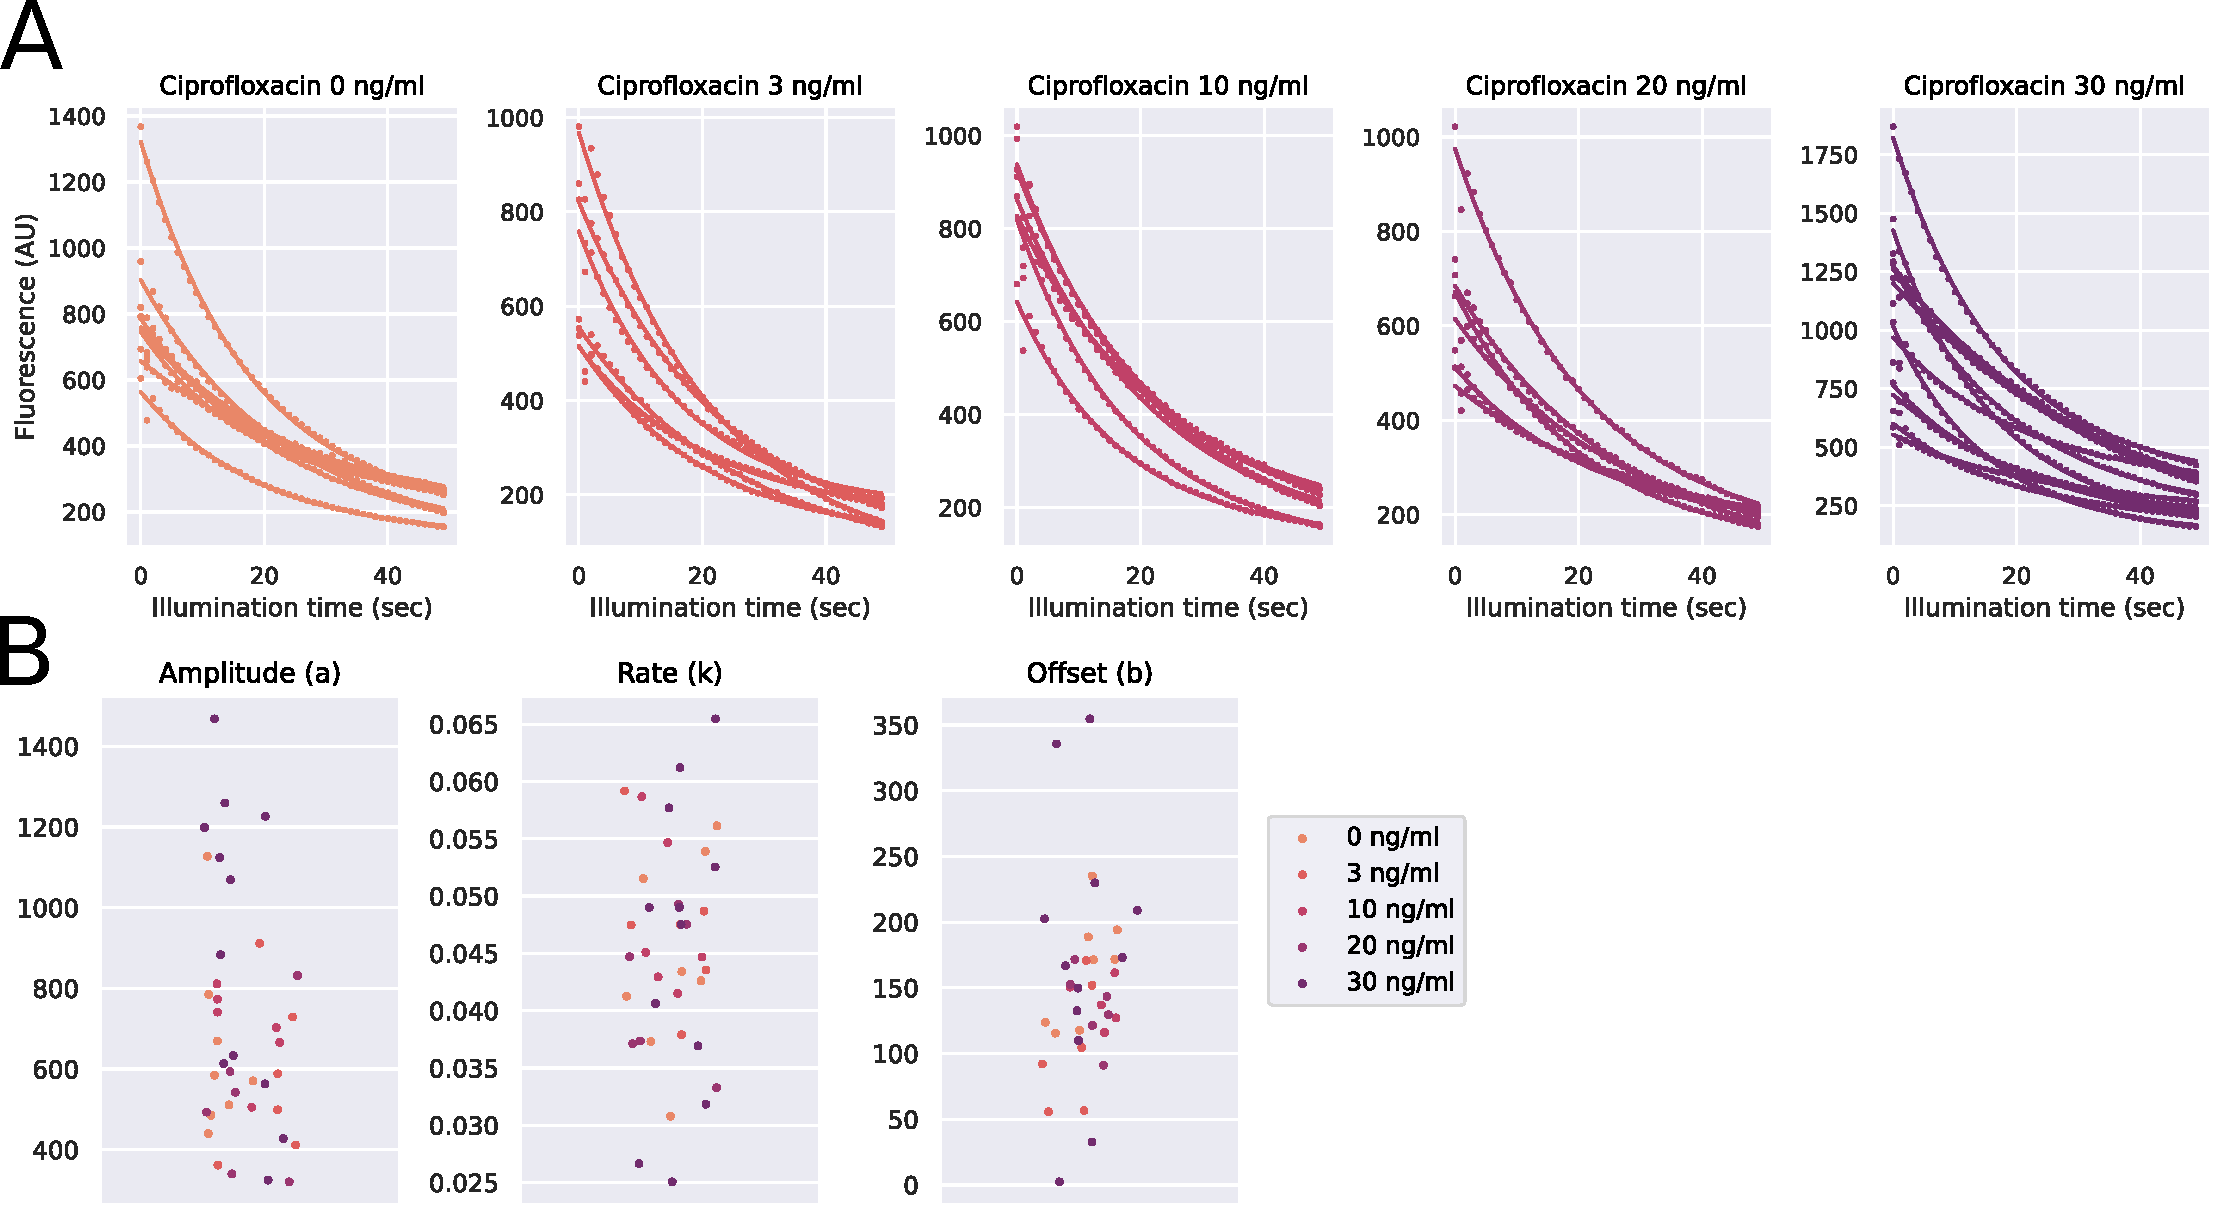
\includegraphics[width=\textwidth]{SI_Figures/SIFig_bleaching.pdf}
    \end{center}
    \caption{Ensemble-level photobleaching of the JF549 dye. \textbf{(A)} Average background-subtracted fluorescence for 5 independent datasets (dots), overlaid with the photobleaching rate fit ($y=a.e^{-k.t}+b$, line) for individual datasets. \ncells{66,764}. \textbf{(B)} Fitted model parameters for each dataset: amplitude (a), photobleaching rate (k) and offset (b). \ncells{66,764}.}
    \label{SIFig:dye_bleaching}
\end{suppfigure*}

% Data analysis pipeline
\begin{suppfigure*}[htbp]
\begin{center}
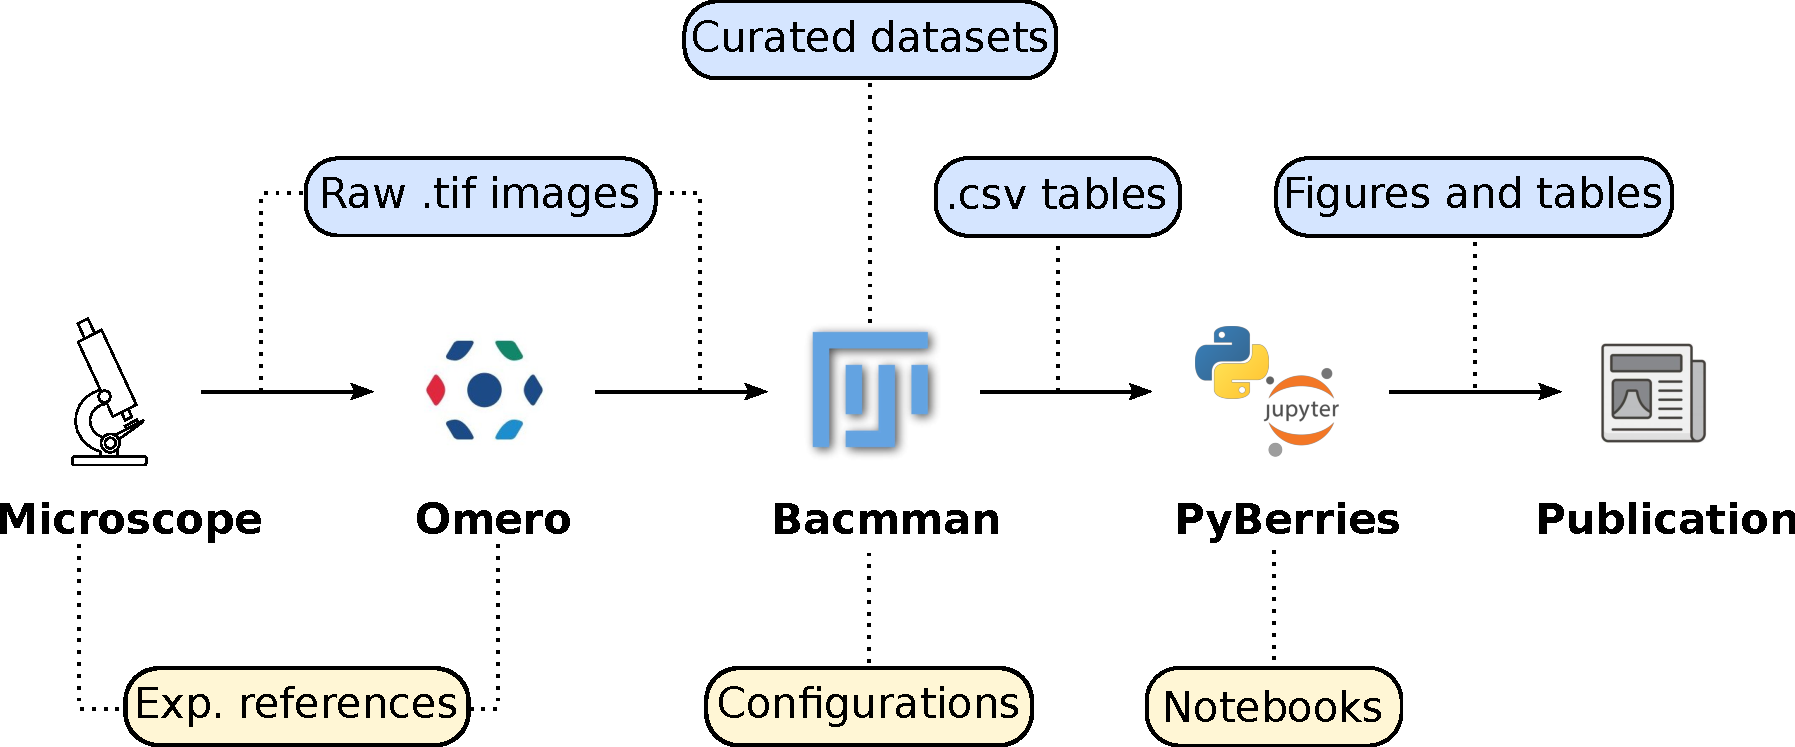
\includegraphics[width=\textwidth]{SI_Figures/Data_analysis_workflow.pdf}
\end{center}
\caption{Data storage and analysis pipeline used in this study. Blue labels indicate stored data and yellow labels indicate code and references that would allow reproducing the different analysis steps.}
\label{SIFig:analysis_workflow}
\end{suppfigure*}

% Object classification workflow
\begin{suppfigure*}[htbp]
    \begin{center}
    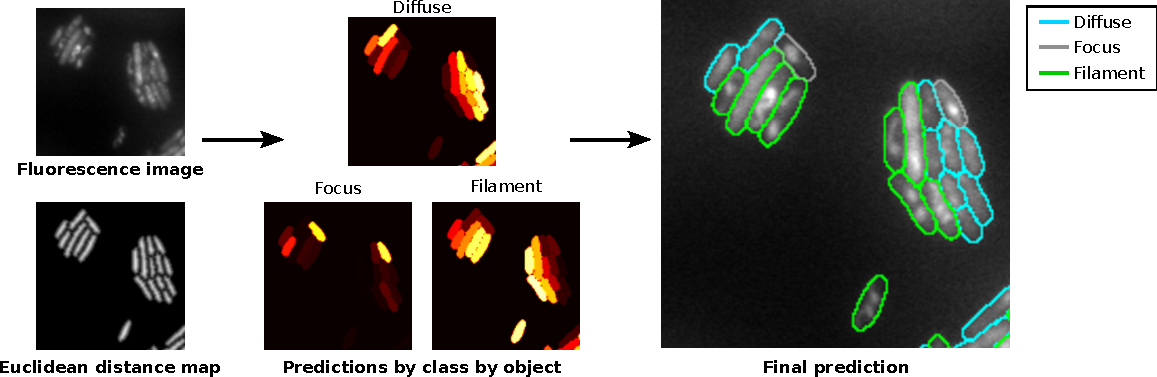
\includegraphics[width=\textwidth]{SI_Figures/ObjectClassifier.pdf}
    \end{center}
    \caption{Classification of cells according to the RecA structures they contain by our in-house Unet-based deep-learning network.}
    \label{SIFig:object_class}
\end{suppfigure*}

% Example image of freely diffusing halo-tag + JF549
\begin{suppfigure*}[htbp]
    \begin{center}
    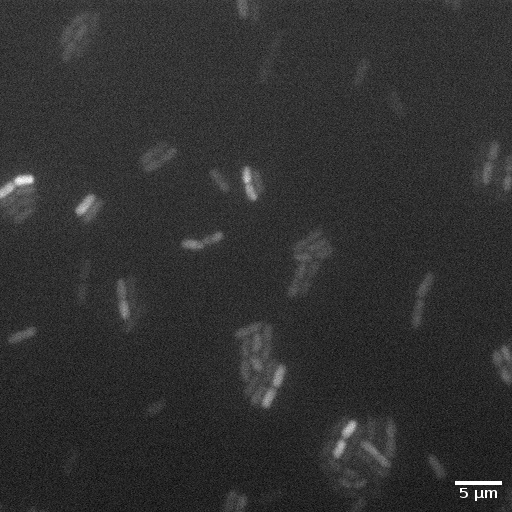
\includegraphics[width=.5\linewidth]{SI_Figures/Free_Halo_image.png}
    \end{center}
    \caption{Representative fluorescence image (1 second exposure time) of freely diffusing Halo-tag expressed from a pBAD plasmid in MG1655 \textit{E. coli} cells.}
    \label{SIFig:freehalo_image}
\end{suppfigure*}

% Example intensity time-traces for single RecB spots
\begin{suppfigure*}[htbp]
    \begin{center}
    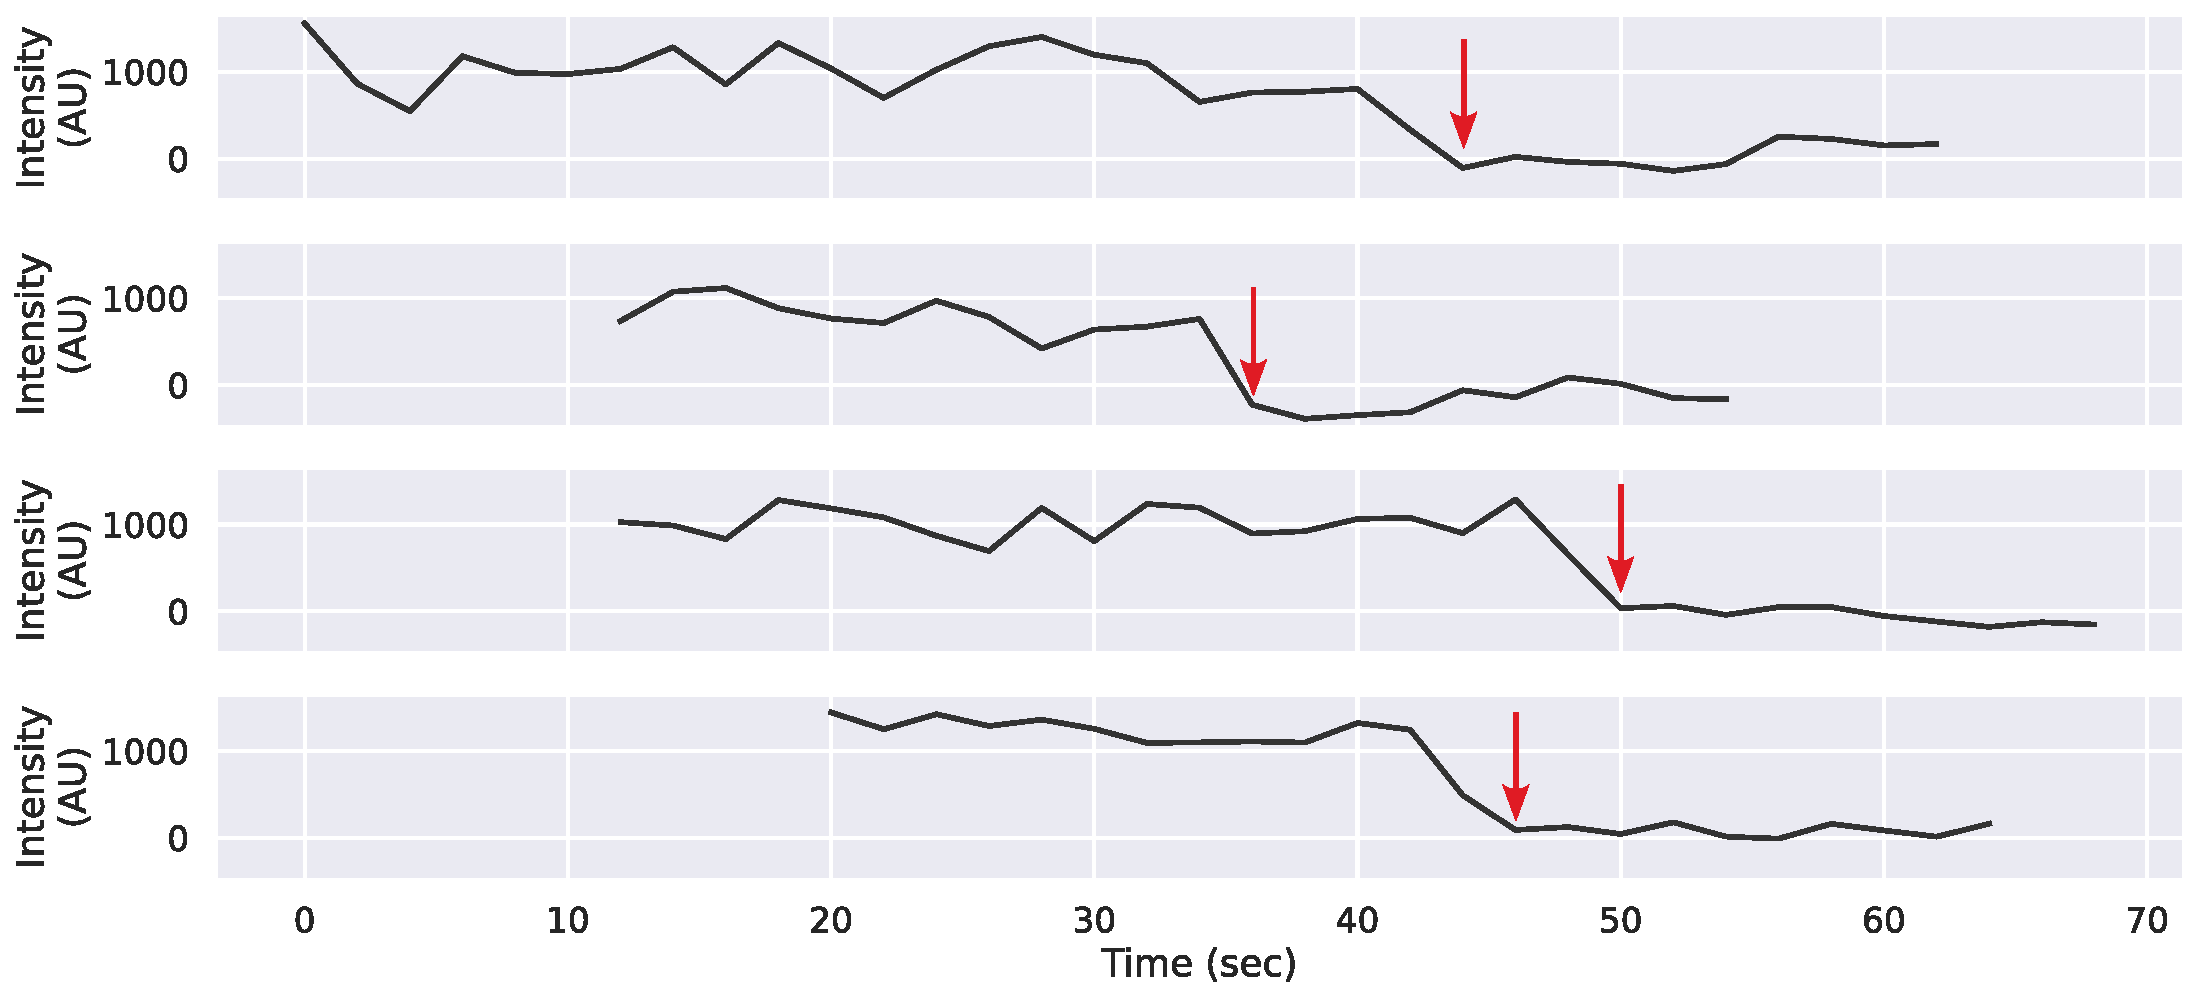
\includegraphics[width=.8\linewidth]{SI_Figures/SM_traces.pdf}
    \end{center}
    \caption{Representative background-subtracted intensity time traces (black lines) for single RecB spots, showing loss of intensity in a single step (red arrows).}
    \label{SIFig:SM_traces}
    \end{suppfigure*}

% Monoexponential fit of WT data, all cipro concentrations
\begin{suppfigure*}[htbp]
    \begin{center}
    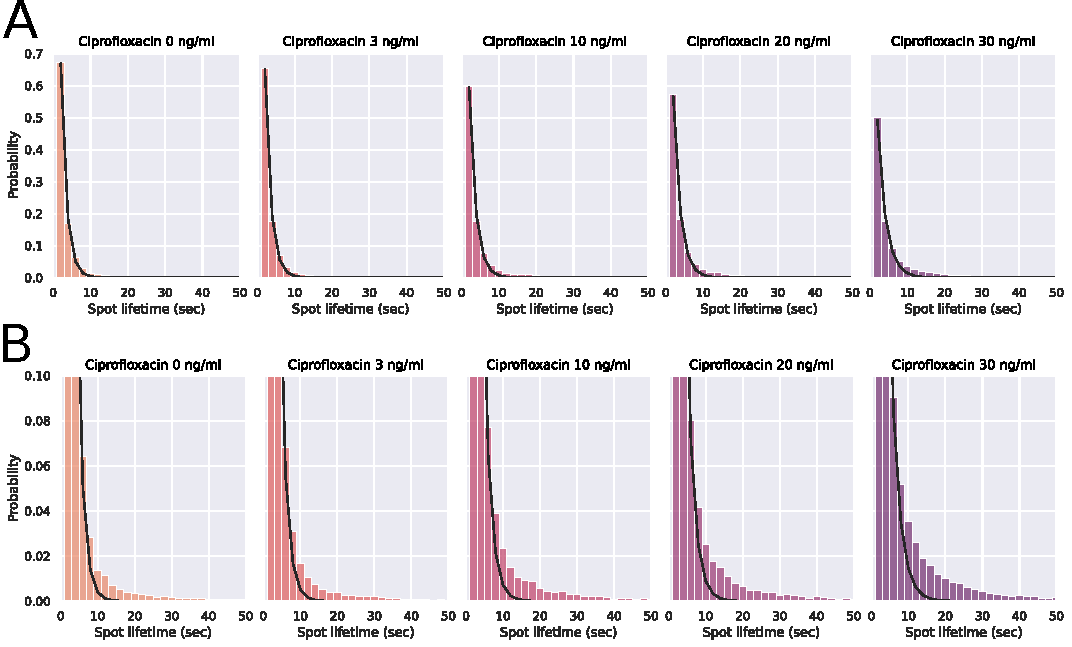
\includegraphics[width=\linewidth]{SI_Figures/Monoexp_fits_cipro.pdf}
    \end{center}
    \caption{\textbf{(A)} Histograms of RecB spot lifetime (bars) under exposure to ciprofloxacin, with overlaid mono-exponential decay fits ($y=a.e^{-k.t}$, black line). \ncells{66,764}. \nspots{170,138} \textbf{(B)} Zoom on the tails of histograms in (A).}
    \label{SIFig:monoexp_fits}
\end{suppfigure*}

% Cell length under Gam over-expression, 0 and 30 ng/mL cipro
\begin{suppfigure*}[htbp]
    \begin{center}
    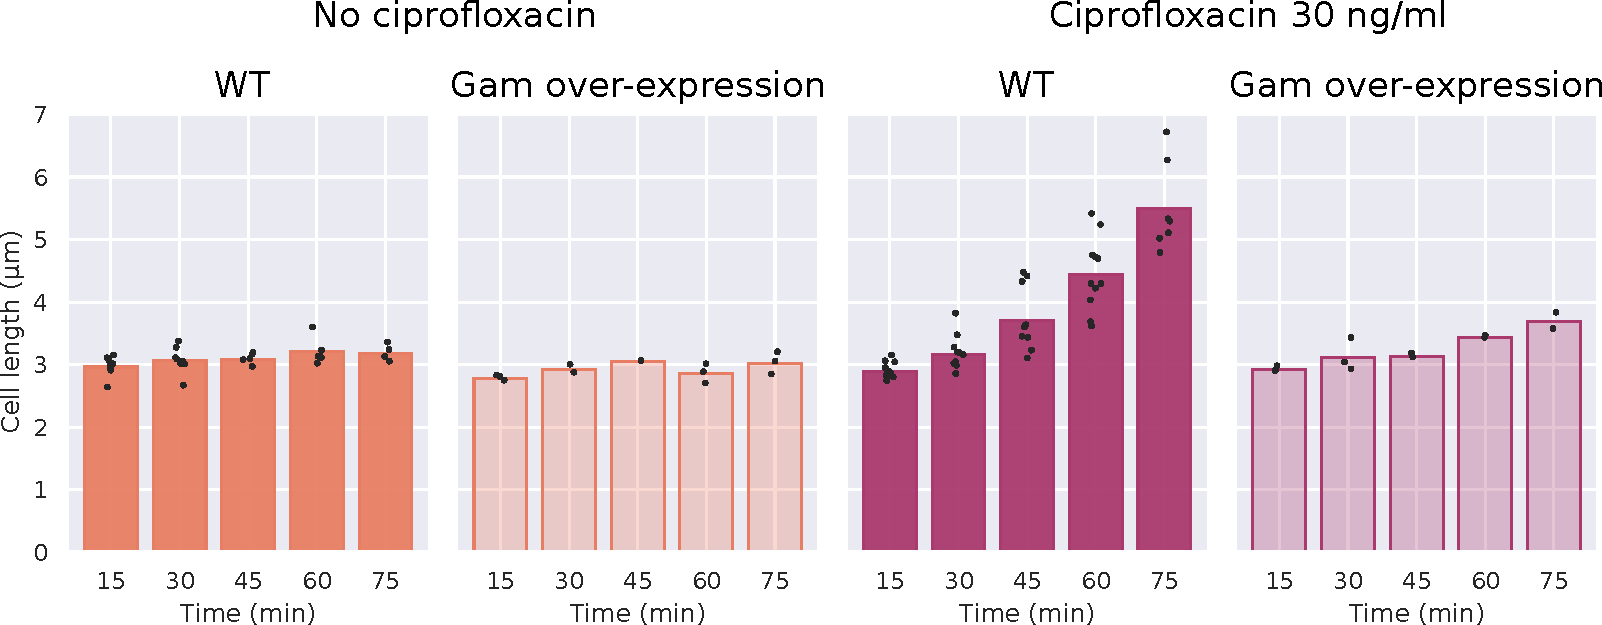
\includegraphics[width=\linewidth]{SI_Figures/Cell_length_Gam.pdf}
    \end{center}
    \caption{Average length of cells that over-express Gam or not (WT), under exposure to 0 or 30 ng/mL ciprofloxacin. Black dots show averages for indvidual datasets, and bars the average between them. \ncells{41,403}.}
    \label{SIFig:Gam_cell_length}
\end{suppfigure*}

% RecB spot lifetimes under Gam over-expression, 0 and 30 ng/mL cipro
\begin{suppfigure*}[htbp]
    \begin{center}
    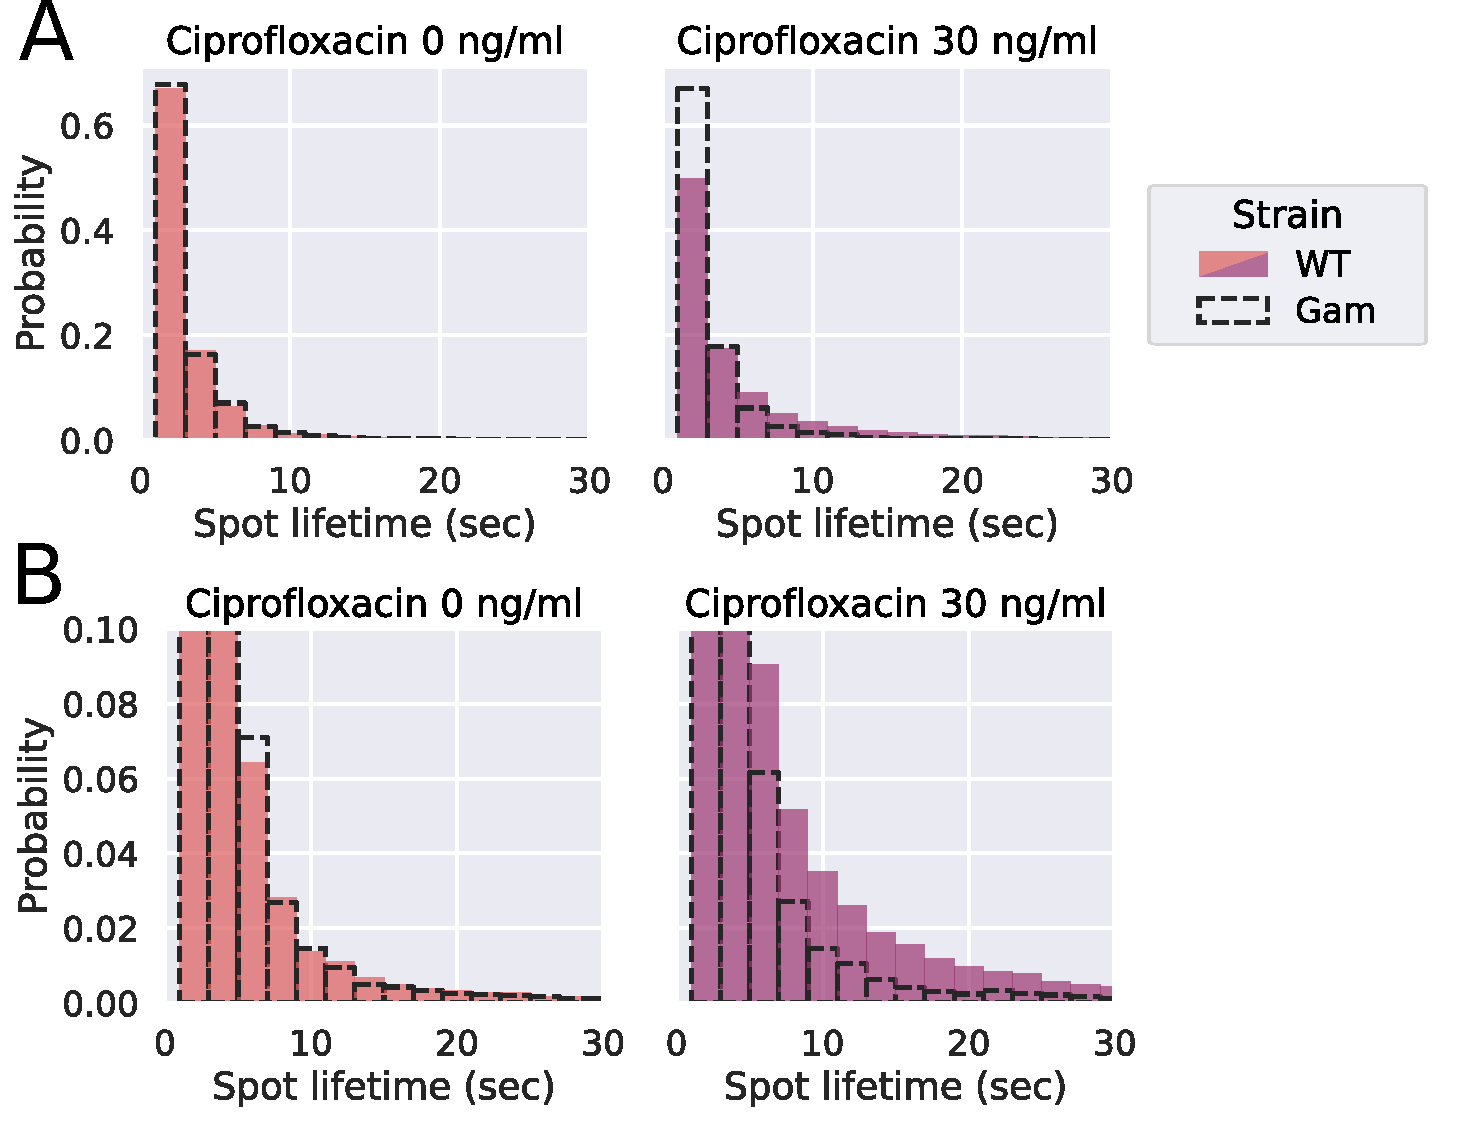
\includegraphics[width=0.75\linewidth]{SI_Figures/Gam_lifetimes_vs_WT.pdf}
    \end{center}
    \caption{\textbf{(A)} Histograms of RecB spot lifetimes for wild-type cells (coloured bars) and cells overexpressing Gam (dashes). \ncells{41,403}. \nspots{96,453} \textbf{(B)} Zoom on the tail of the histograms from (A).}
    \label{SIFig:Gam_RecB_lifetimes_vs_WT}
\end{suppfigure*}

% Displacements simulation
\begin{suppfigure*}[htbp]
    \begin{center}
    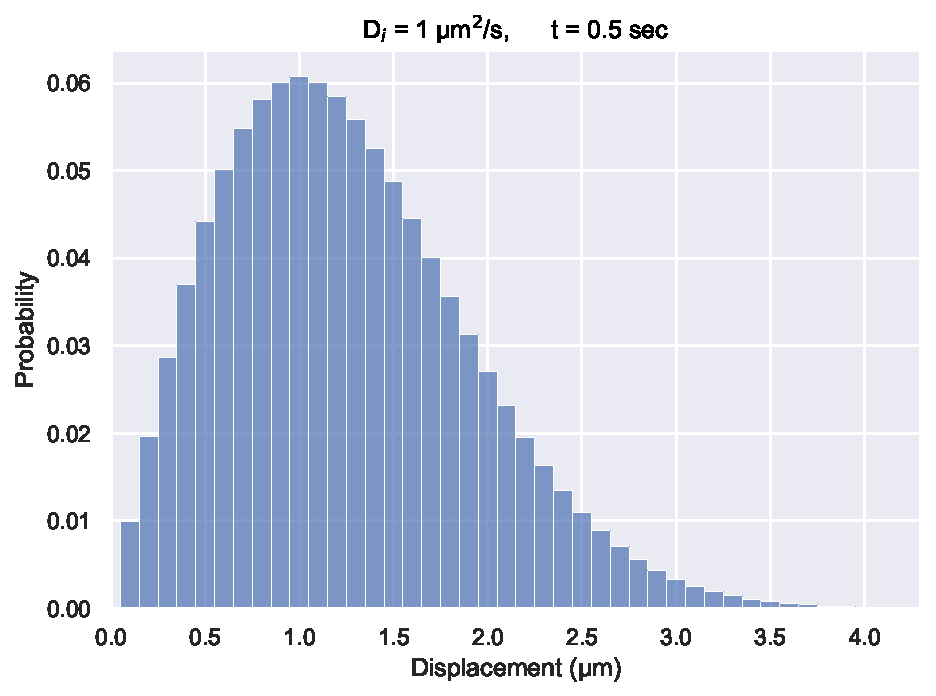
\includegraphics[width=.8\textwidth]{SI_Figures/Displacements_distribution.pdf}
    \end{center}
    \caption{Histogram of expected displacements for a molecule diffusing at 1 \ums\ over a 500 ms frame time.}
    \label{SIFig:displacement_simul}
\end{suppfigure*}

% Fitted RecB spot lifetimes at different durations of ciprofloxacin exposure
\begin{suppfigure*}[htbp]
    \begin{center}
    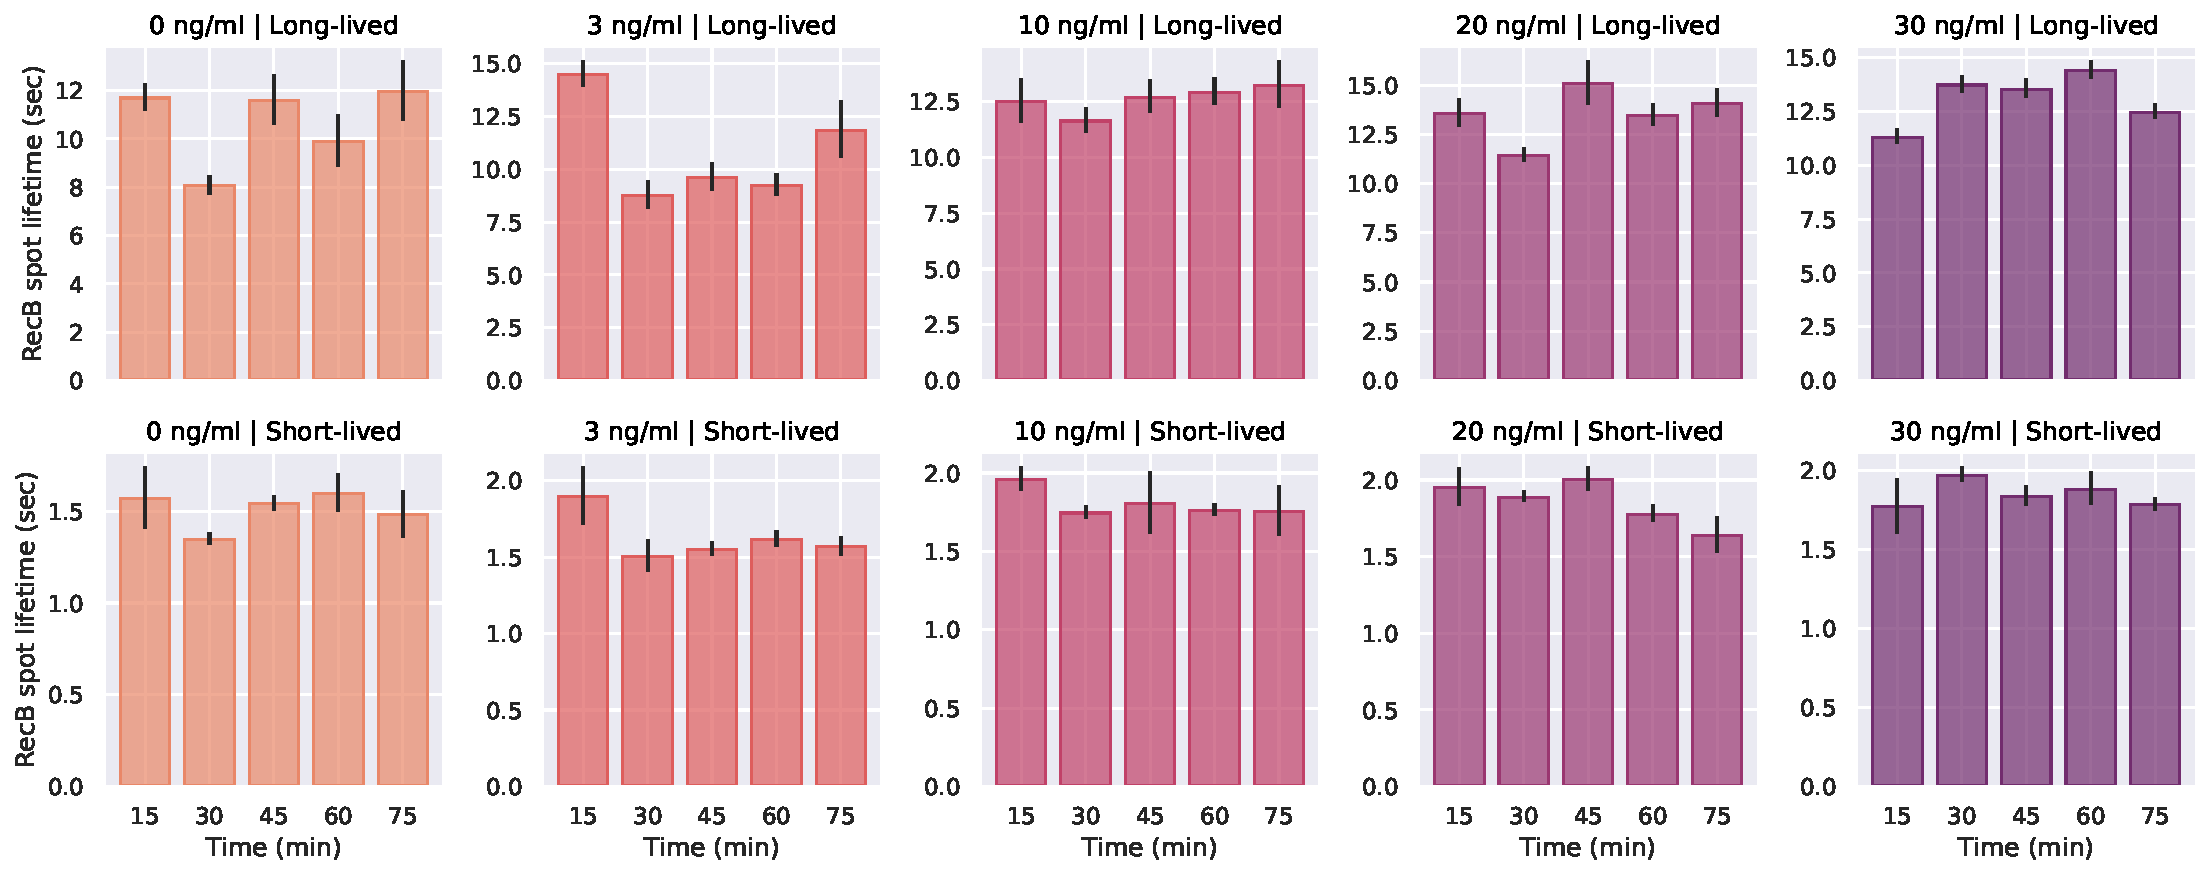
\includegraphics[width=.7\linewidth]{SI_Figures/RecB_lifetime_timepoints.pdf}
    \end{center}
    \caption{Fitted lifetimes of short- and long-lived RecB spots, following different durations of exposure to 30 ng/ml ciprofloxacin. Coloured bars represent the fitted lifetimes, and black strokes the standard error of the mean obtained by bootstrapping. \ncells{18,945}. \nspots{54,475}}
    \label{SIFig:RecB_lifetimes_timepoints}
    \end{suppfigure*}

% Mutants: RecB spot lifetime histogram bi-exp fits
\begin{suppfigure*}[htbp]
    \begin{center}
    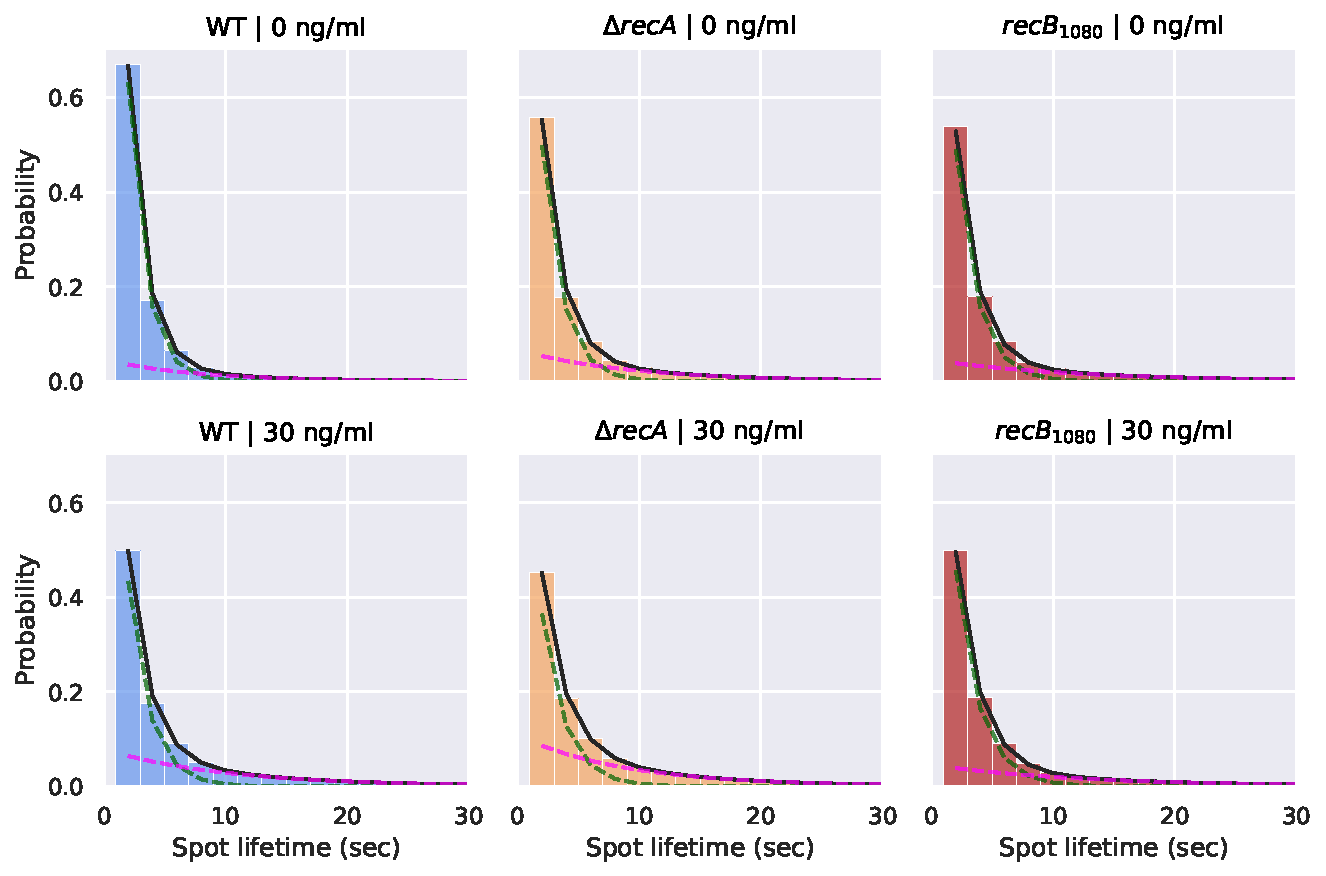
\includegraphics[width=.8\textwidth]{SI_Figures/Mutants_RecB_fits.pdf}
    \end{center}
    \caption{RecB spot lifetime histograms for wild-type (WT), \dreca and \geneteneighty\ mutants, at 0 and 30 ng/mL ciprofloxacin, fitted with a bi-exponential decay model (black line, fit components showed as dashed lines). \ncells{56,131}. \nspots{177,646}.}
    \label{SIFig:mutants_biexp_fits}
\end{suppfigure*}

% Effect of DSBs on the cell: nucleoid compaction
\begin{suppfigure*}[htbp]
    \begin{center}
    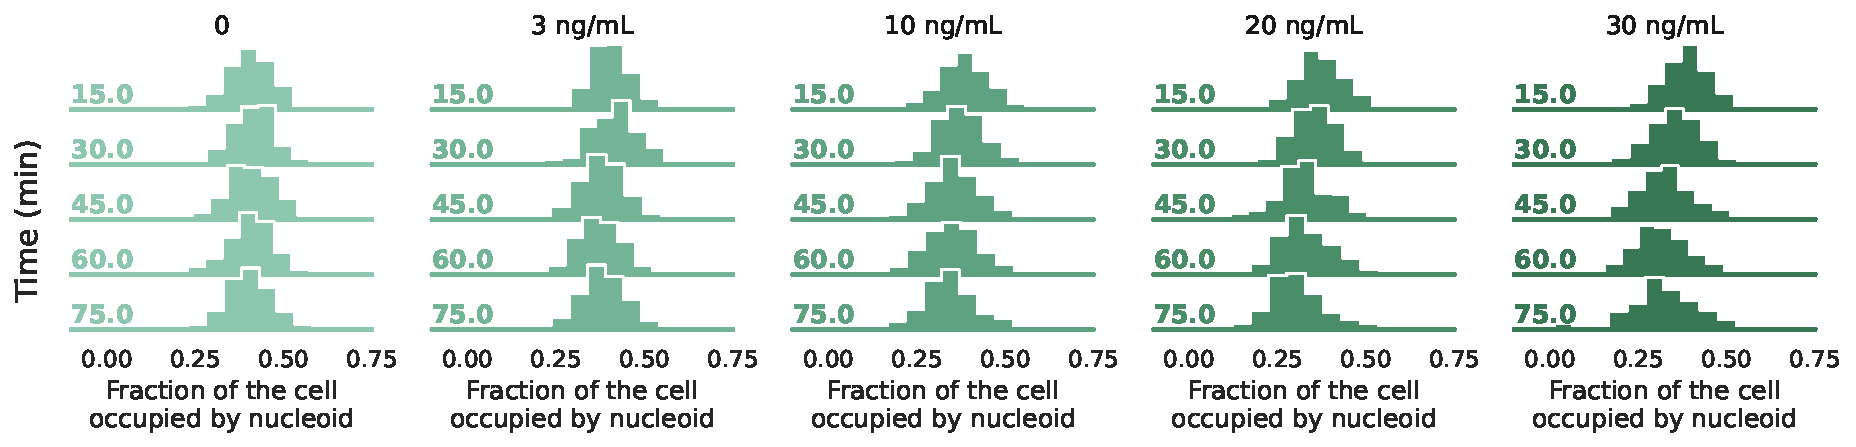
\includegraphics[width=\textwidth]{SI_Figures/Nucleoid_compaction.pdf}
    \end{center}
    \caption{Average fraction of the bacterial cell occupied by the nucleoid (stained using the Sytox Green dye) at different ciprofloxacin concentrations (0 to 30 ng/ml) and duration of exposure (15 to 75 min). Dots represent averages for individual datasets, and dashes the average between them. \ncells{24,014}. \nnucl{31,441}.}
    \label{SIFig:nucleoid_compaction}
\end{suppfigure*}

% Effect of DSBs on the cell: nucleoid position
\begin{suppfigure*}[htbp]
    \begin{center}
    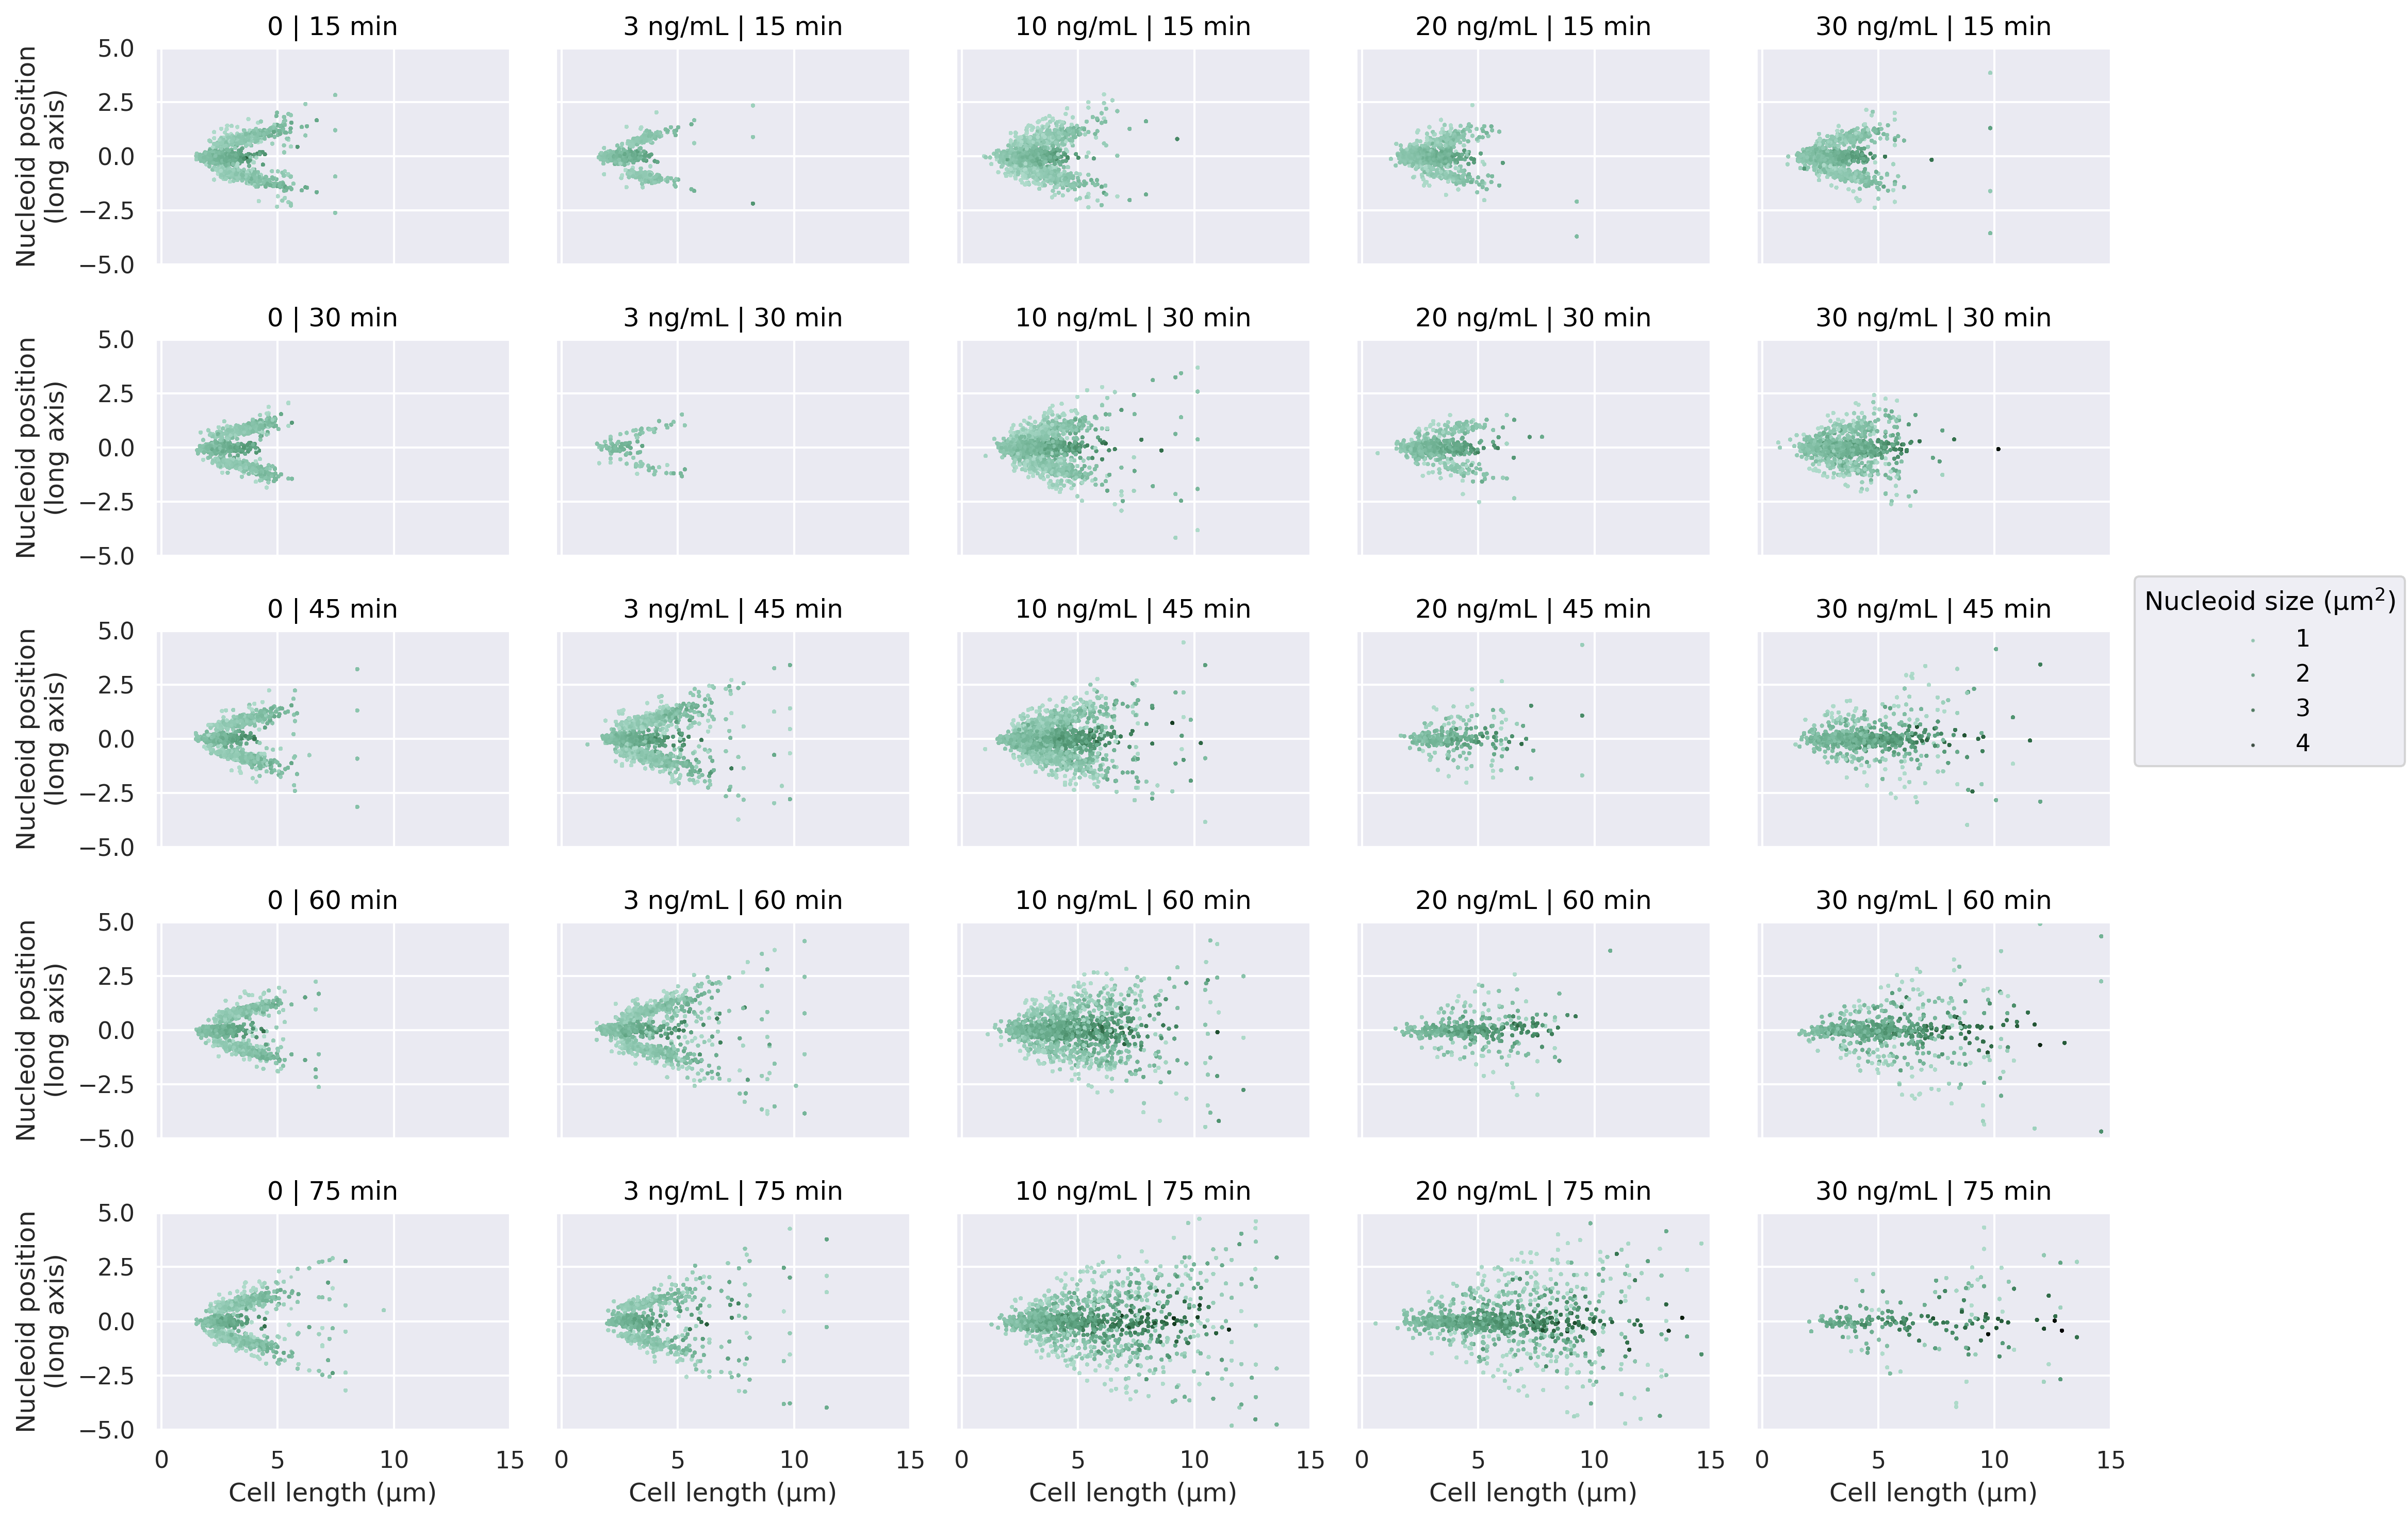
\includegraphics[width=\textwidth]{SI_Figures/Nucleoid_position.png}
    \end{center}
    \caption{Position of the nucleoid along the cell's long axis against cell length for different ciprofloxacin concentrations (columns) and durations of ciprofloxacin exposure (rows). Point colour indicates the total surface covered by the nucleoid in the cell, in \umsq. \ncells{24,014}. \nnucl{31,441}.}
    \label{SIFig:nucleoid_position}
\end{suppfigure*}

% Effect of DSBs on the cell: nucleoid and RecB position overlay separated by timepoints
\begin{suppfigure*}[htbp]
    \begin{center}
    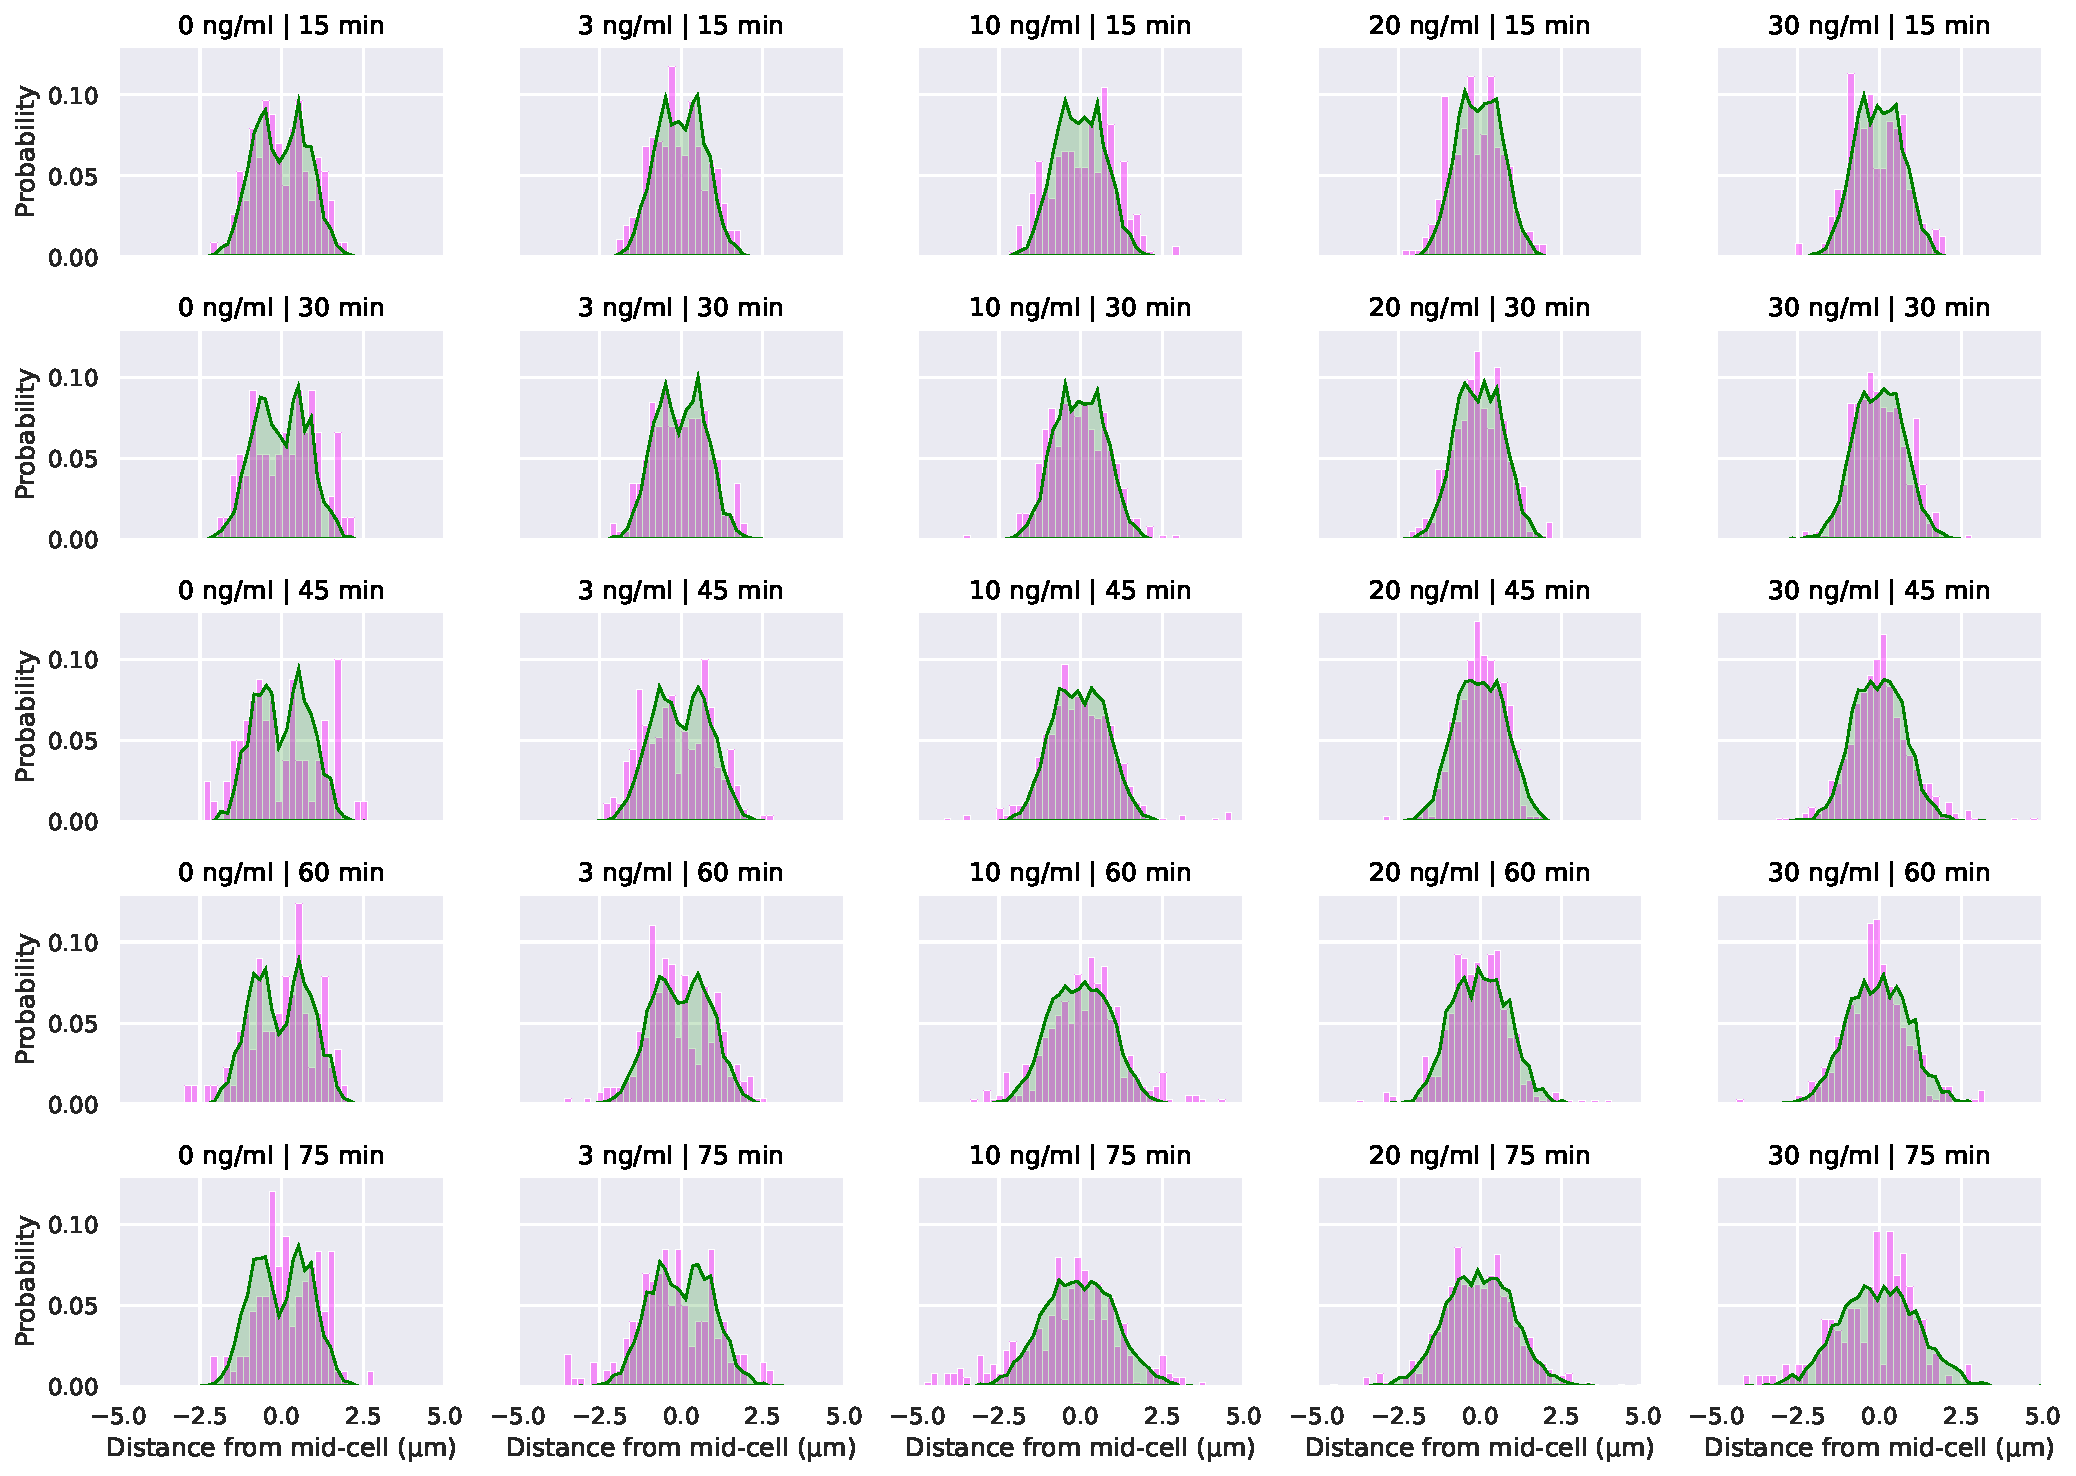
\includegraphics[width=\textwidth]{SI_Figures/RecB_Nucleoid_position_timepoints.pdf}
    \end{center}
    \caption{Overlay of nucleoid density (green area) and position of DSB-bound RecB molecules (magenta bars) along the cell's long axis, for different ciprofloxacin concentrations (columns) and durations of exposure (rows). \ncells{15,029}. \nspots{58,331}. \nnucl{20,831}.}
    \label{SIFig:recb_nucleoid_timepoints}
\end{suppfigure*}

% Mutants: nucleoid compaction
\begin{suppfigure*}[htbp]
    \begin{center}
    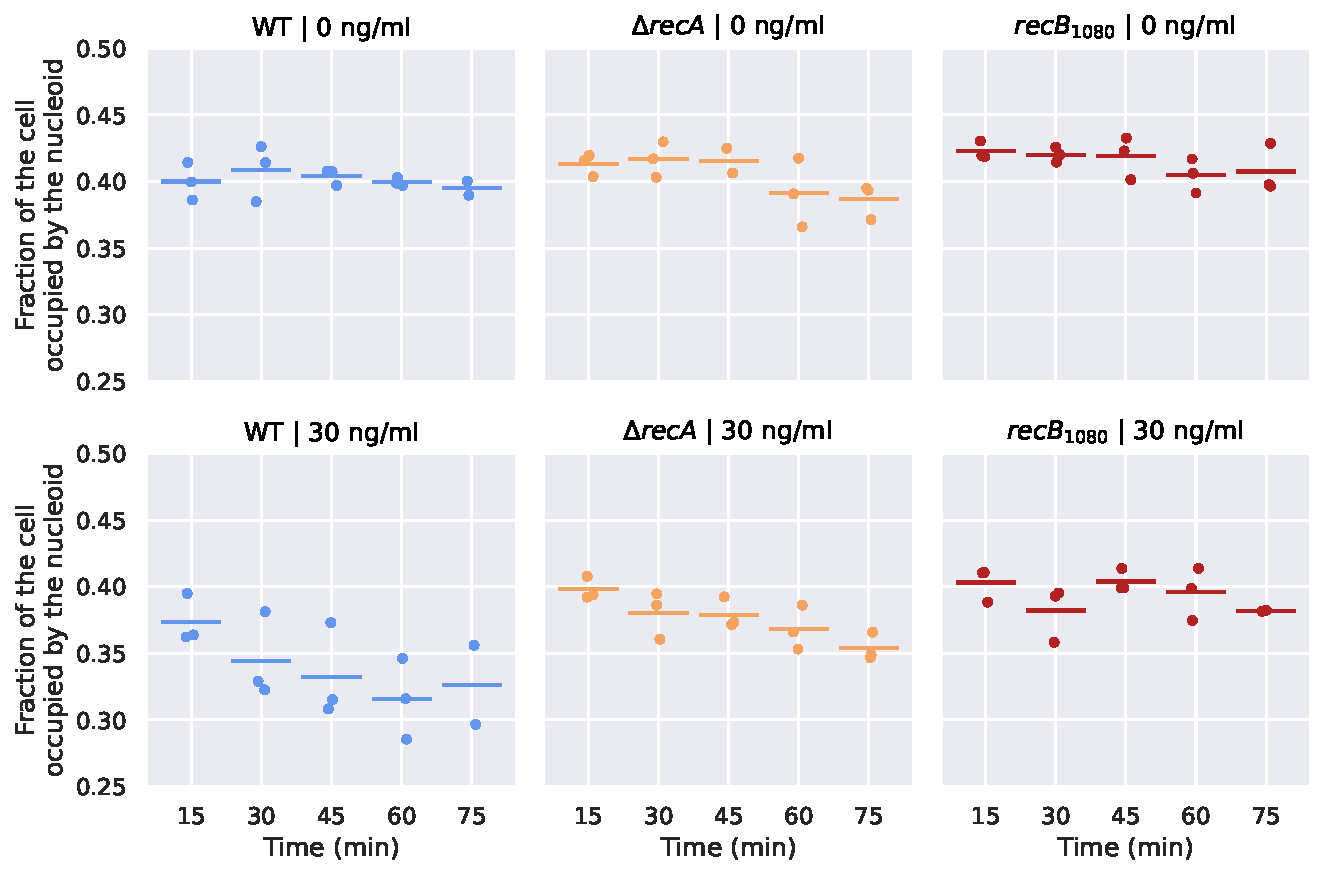
\includegraphics[width=.8\textwidth]{SI_Figures/Mutants_nucleoid_compaction.pdf}
    \end{center}
    \caption{Average fraction of the bacterial cell occupied by the nucleoid (stained using the Sytox Green dye) at different ciprofloxacin concentrations (0 to 30 ng/mL) and duration of exposure (15 to 75 min), for wild-type cells (reproduced from Supp. Figure \ref{SIFig:nucleoid_compaction} for comparison) and the \dreca\ and \geneteneighty\ mutants. Dots represent averages for individual datasets, and dashes the average between them. \ncells{15,029}. \nnucl{20,831}.}
    \label{SIFig:mutants_nucleoid_compaction}
\end{suppfigure*}

% RecA structures
\begin{suppfigure*}[htbp]
    \begin{center}
    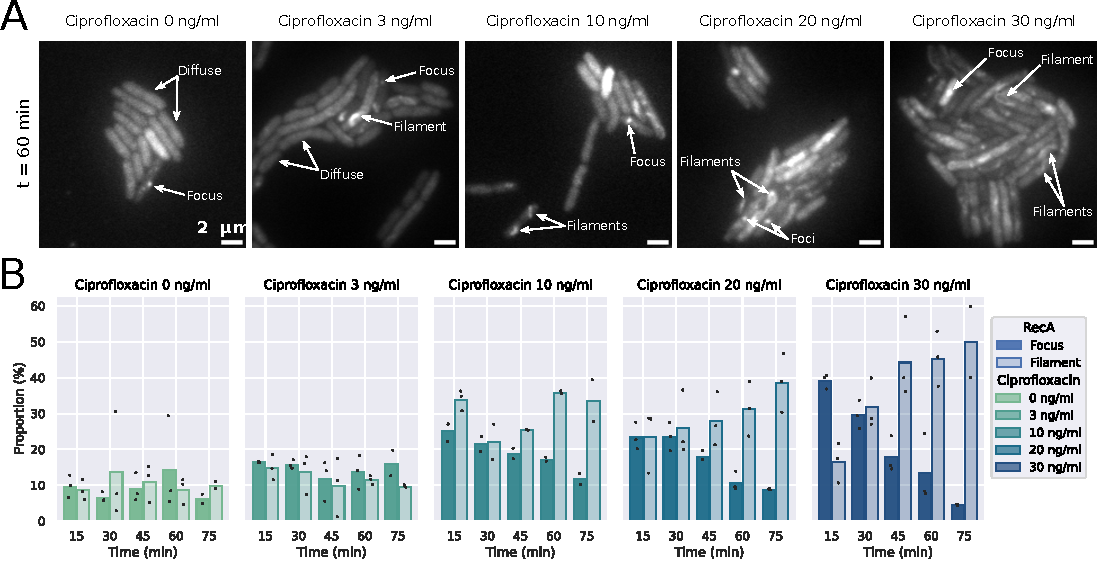
\includegraphics[width=\textwidth]{SI_Figures/RecA_structures.pdf}
    \end{center}
    \caption{RecA structures formed upon exposure to ciprofloxacin. \textbf{(A)} Representative images of cells containing different RecA structures (diffuse fluorescence, foci or filaments) after 60 minutes of exposure to ciprofloxacin. Arrows point to representative examples of each of these structures. \textbf{(B)} Proportion of cells containing RecA foci or filaments. Black dots represent averages for individual datasets, and bars the average between them. \ncells{32,031}.}
    \label{SIFig:reca_structures}
\end{suppfigure*}
